\documentclass[tikz,crop]{standalone}

\usepackage{tikz}
\usetikzlibrary{arrows,calc,shapes.geometric, backgrounds, positioning}
\usepackage{siunitx}

\definecolor{master453}{RGB}{0, 87, 255}
\definecolor{slave441}{RGB}{0, 11, 255}

\pgfdeclarelayer{background}
\pgfdeclarelayer{foreground}
\pgfsetlayers{background,main,foreground}

\tikzstyle{laser} = [rectangle, draw, thick, fill=blue!25, text width=10em, text badly centered, rounded corners, minimum height=4em]
\tikzstyle{controller} = [rectangle, draw, thick, fill=orange!25, text width=10em, text badly centered, rounded corners, minimum height=4em]
\tikzstyle{line} = [draw, line width=2.5, -latex]

\begin{document}
    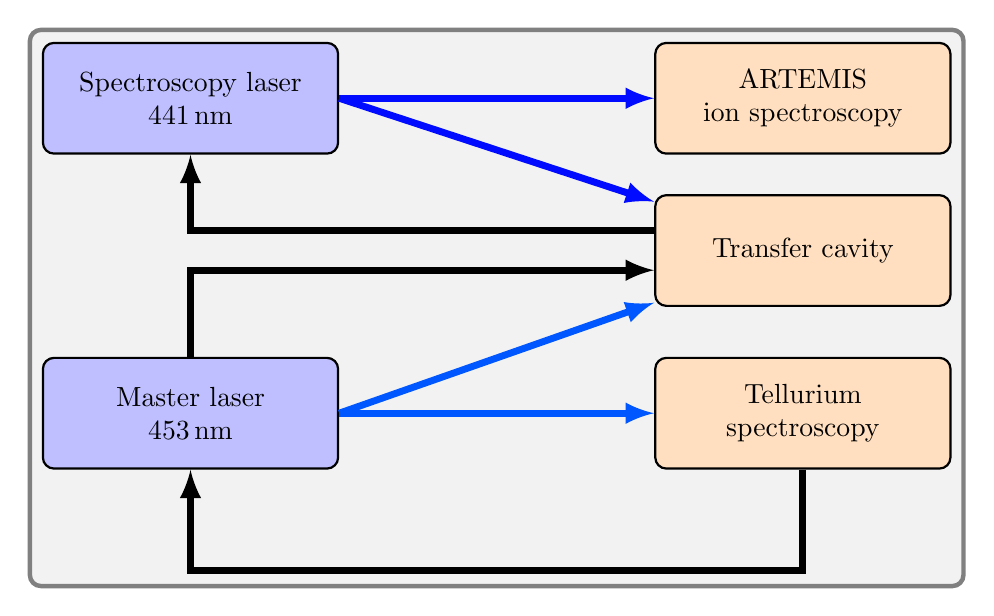
\begin{tikzpicture}[%
        node distance=0.5cm and 4cm,%
        auto,%
        background rectangle/.style={fill=gray!10, rounded corners, ultra thick,draw=gray},%
        show background rectangle,%
    ]
        \node[laser] (master) at (0,0) {Master laser\\\qty{453}{\nm}};
        \node[laser] (slave) at (0,4) {Spectroscopy laser\\\qty{441}{\nm}};
        \node[controller, right=of master] (spectroscopy) {Tellurium spectroscopy};
        \node[controller, right=of slave] (experiment) {ARTEMIS\\ion spectroscopy};
        \node[controller, below=of experiment] (cavity) {Transfer cavity};
        %\node[block,text width=10em]  (kraken) at (0,4) {Spectroscopy laser\\\qty{441}{\nm}};
        % Arrows
        \path [line, master453] (master) -- (spectroscopy);
        \path [line, master453] (master.east) -- (cavity);
        \path [line, black] (master) |- ($(cavity.west) -(0,0.25)$);
        \path [line, black] (cavity.west) ++(0,0.25) -| (slave);
        \path [line, black] (spectroscopy) -- ++(0,-2) -| (master);
        \path [line, slave441] (slave) -- (experiment);
        \path [line, slave441] (slave.east) -- (cavity);
        %\path [line,rounded corners] (calculate) |- ($(calculate.south east) + (0.5,-0.5)$) |- (signal);
    \end{tikzpicture}
\end{document}
